%Umfrage
\section{Nutzerstudie}
Im Rahmen der Bedürfnissermittlung wurde eine Nutzerstudie durchgeführt. Im Rahmen einer Onlineumfrage wurden 170 Personen (Stand: 27.05.2020) nach ihren Präfernezen und Hauptinteressen gefragt. Im folgenden werden die Ergebnisse vorgestellt.
Alle vorgestellten Ergebnisse beziehen sich auf den Stand der Studie am 27.05.2020\\

\subsection{Alterverteilung}
In der Umfrage wurde das Geburtsjahr der Teilnehmer abgefragt. Dies trägt dazu bei, die Nutzergruppe geneuer einschätzen zu können.
\\
\begin{figure}[h]
    \centering
    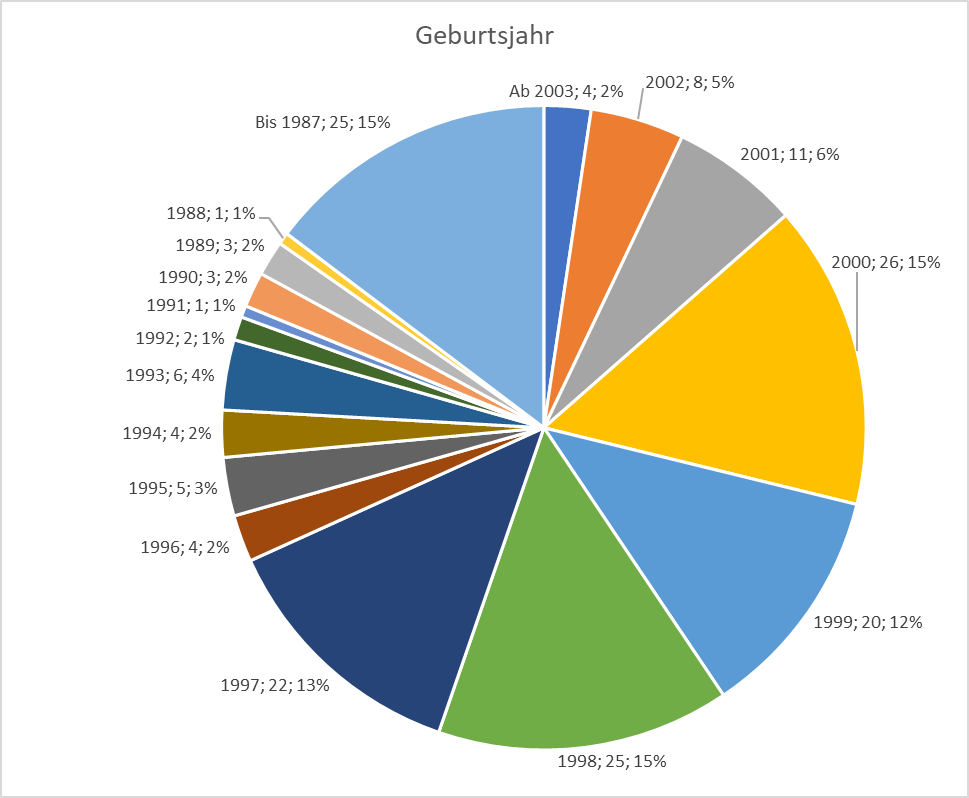
\includegraphics[width=0.7\textwidth]{media/diagram/geburtsjahr.png}
    \caption{Verteilung der Geburtsjahre der Befragten}
\end{figure}
\\
\subsection{Selbsteinschätzung von Wissen und Interesse am Thema Luftverschmutzung}
Für eine beurteilung des Interesses an den in \softwarename gezeigten Informationen wurde nach dem Interesse auf der Seite der nutzer gefragt.
Um abzuschätzen wie viel wissen bereits über Luftverschmutzung vorhanden ist wurde gefragt, wie die Nutzer ihr eigenes Wissen über Luftverschmutzung einschätzen.
\\
Bei beiden Einschätzungen wurde jeweils eine Zahl zwischen 1 und 5 abgefragt, wobei 1 sehr wichtig und 5 sehr unwichtig ist.
\\
\begin{figure}[h]
    \subfigure[Einschätzung zum eigenen Wissen über Luftverschmutzung]{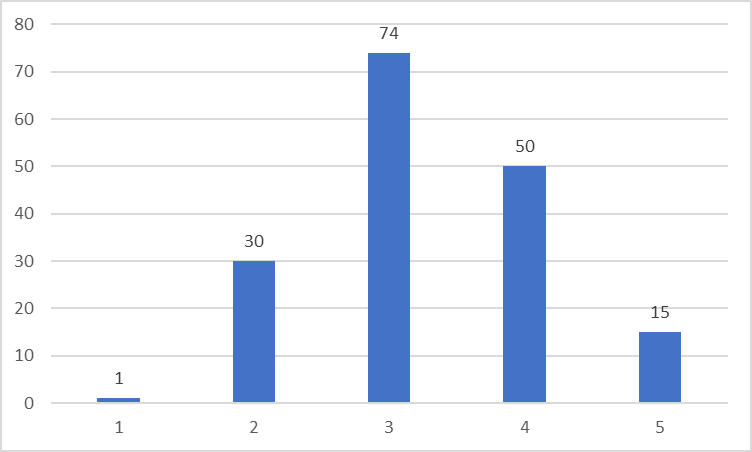
\includegraphics[width=0.49\textwidth]{media/diagram/eigenesWissen.png}}
    \subfigure[Einschätzung zur wichtigkeit von Informationen über Luftverschmutzung]{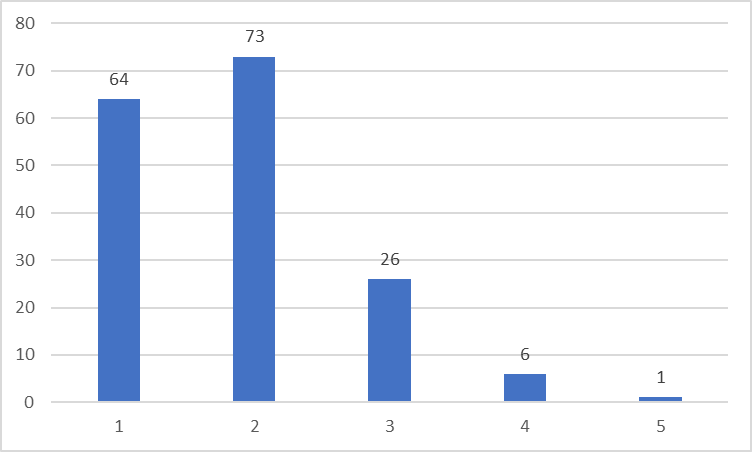
\includegraphics[width=0.49\textwidth]{media/diagram/WichtigkeitVonInfos.png}}
    \caption{Selbsteinschätzung der Nutzer}
\end{figure}
\\
Weiter wurden die Nutzer gefragt wie sie ihre Informationen zum Thema Luftverschmutzung erhalten. Die verbreitesten Informationsquellen sind hierbei
\begin{itemize} [noitemsep]
    \item Nachrichtensendungen und Berichterstattungen (circa 79\%)
    \item Informationen aus dem Internet (circa 78 \%)
    \item Gespräche mit anderen Personen (circa 26 \%)
\end{itemize}
Daraus ergibt sich, dass eine Webseite für die Vermittlung gut geeignet ist, da dieses Medium bereits weit verbreitet ist.

\subsection{Einschätzung zu Aufrufen der Webseite}
Die Teilnehmer wurden gefragt wie oft sie eine Webseite mit Luftqualitätsdaten aufrufen würden.
\\
\begin{figure}[h]
    \centering
    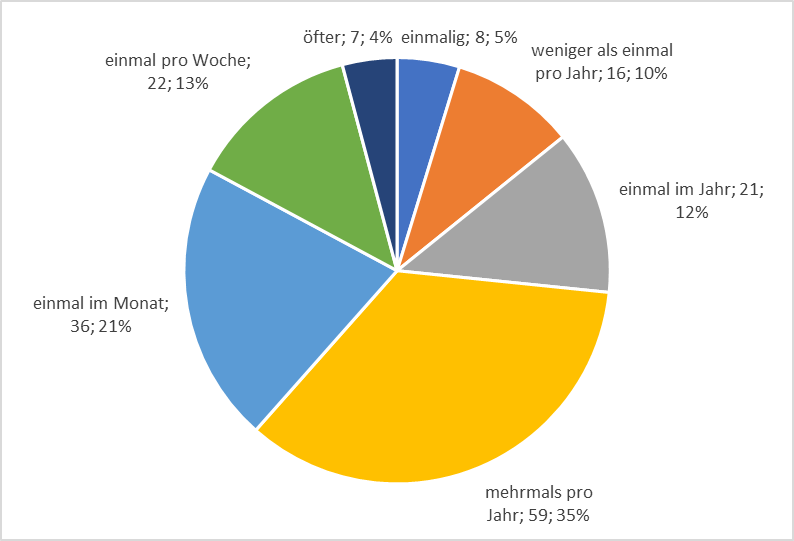
\includegraphics[width=0.7\textwidth]{media/diagram/aufrufe.png}
    \caption{Geschätzte Häufigkeit der Aufrufe}
\end{figure}
\\
Dieser Parameter ist hilfreich um die Last auf die Webseite abzuschätzen
\\
Die häufigsten Gründe für den Aufruf einer solchen Webseite sind laut der Nutzerstudie
\begin{itemize} [noitemsep]
    \item Information vor Schul- oder Hausarbeiten
    \item Generelles Interesse
    \item Verifikation von Gerüchten
    \item Vor Reisen oder Wohnortswechsel
\end{itemize}
Die Geräte von welchen die Webseite im wesentlichen aufgerufen wird sind.
\begin{itemize} [noitemsep]
    \item Smartphones
    \item Tabletts
    \item PCs
    \item Laptops
\end{itemize}

\subsection{Art des Informationsbedürfnisses}
Gefragt wurde wie wichtig die Luftverschmutzung in welcher Region für die Teilnehmer ist.
Viele Teilnehmer der Studie interessieren sich für die Luftverschmutzung in ihrer eigenen Region. Auch finden viele Informationen über Luftverschmutzung in Deutschland im Überblick wichtig. Weniger wichtig finden die Nutzer hingegen die Luftverschmutzung in anderen Regionen.
\\
\begin{figure}[h]
    \centering
    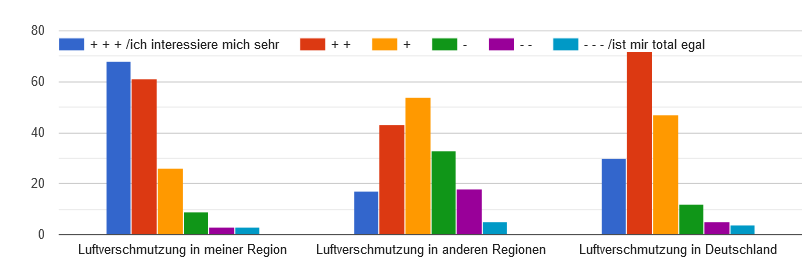
\includegraphics[width=1\textwidth]{media/diagram/interesse.png}
    \caption{Interesse der Nutzer an der Luftverschmutzung in verschiedenen Regionen}
\end{figure}
\\
Weiter gaben die Teilnehmer an,  dass sowohl die Auswirkungen von Luftverschmutzung und die Ursachen von Luftverschmutzung sehr wichtig sind. Eher weniger wichtig sind die Messmethoden der Luftverschmutzung
\\
\begin{figure}[h]
    \centering
    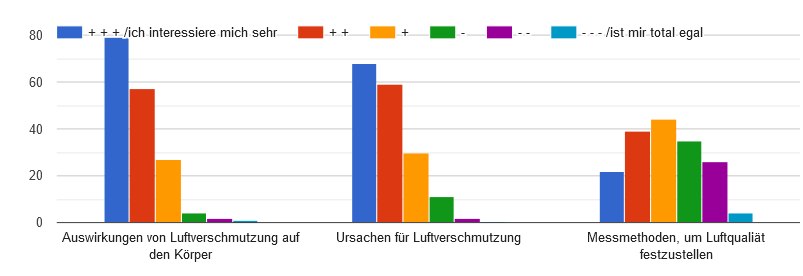
\includegraphics[width=1\textwidth]{media/diagram/interesse2.png}
    \caption{Interesse der Nutzer an Zusatzinformationen zu Luftverschmutzung}
\end{figure}
\\
Auch ergab sich, dass sowohl die zeitliche Entwicklung der Luftqualitätsdaten als auch die momentane Luftqualität etwa gleich wichtig sind. Interesse am Bau von \gls{DIY}-\glspl{Sensor} zeigen etwa 40\%  der Teilnehmer.
Über die hälfte der Nutzer gab an, dass die Vergleiche von regionaler Luftverschmutzung mit der Belastung der Luft durch einzelne technische Geräte sehr hilfreich finden würden.
\\
Als besonders wichtig hoben viele Teilnehmer die Übersichtlichkeit und die benutzbarkeit für Laien hervor.

\subsection{Darstellungsweisen von Luftverschmutzung}
Gefragt wurde zusätzlich welche Darstellungsform die Teilnehmer am ansprechend finden.
\begin{figure}[h]
    \centering
    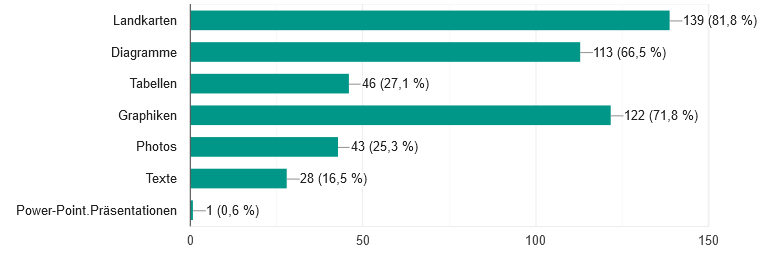
\includegraphics[width=1\textwidth]{media/diagram/darstellung.png}
    \caption{Präferenzen bei der Darstellung von Luftverschmutzung}
\end{figure}
